% !TEX program = xelatex
\documentclass[a4paper,14pt,oneside,openany]{memoir}

%%% Задаем поля, отступы и межстрочный интервал %%%

\usepackage[left=30mm, right=15mm, top=20mm, bottom=20mm]{geometry}
\pagestyle{plain}
\parindent=1.25cm
\usepackage{indentfirst}

%%% Задаем языковые параметры и шрифт %%%

\usepackage[english,russian]{babel}
\babelfont[russian]{rm}{Times New Roman}
\babelfont[russian]{tt}{Courier New}

%%% Задаем стиль заголовков и подзаголовков в тексте %%%

\setsecnumdepth{subsection}
\renewcommand*{\chapterheadstart}{}
\renewcommand*{\printchaptername}{}
\renewcommand*{\chapnumfont}{\normalfont\bfseries}
\renewcommand*{\afterchapternum}{\hspace{1em}}
\renewcommand*{\printchaptertitle}[1]{\normalfont\bfseries\centering\MakeUppercase{#1}}
\setbeforesecskip{20pt}
\setaftersecskip{20pt}
\setsecheadstyle{\raggedright\normalfont\bfseries}
\setbeforesubsecskip{20pt}
\setaftersubsecskip{20pt}
\setsubsecheadstyle{\raggedright\normalfont\bfseries}

%%% Исправление нумерации секций %%%

\renewcommand{\thesection}{\arabic{section}}
\renewcommand{\thesubsection}{\arabic{subsection}}

%%% Сквозная нумерация рисунков и таблиц %%%

\counterwithout{figure}{chapter}
\counterwithout{table}{chapter}

%%% Выравнивание и переносы %%%

\tolerance 1414
\hbadness 1414
\emergencystretch 1.5em
\clubpenalty=10000
\widowpenalty=10000

%%% Задаем параметры оформления рисунков и таблиц %%%

\usepackage{graphicx}
\usepackage{caption}
\usepackage{subcaption}
\usepackage{float}
\graphicspath{{photo/}}
\captionsetup[figure]{font=small, width=\textwidth, name=Рисунок, justification=centering}
\captiondelim{ --- }
\usepackage[section]{placeins}

%%% Задаем параметры ссылок и гиперссылок %%% 

\usepackage{hyperref}
\hypersetup{
    colorlinks=true,
    linkcolor=red,
    citecolor=red
}

%%% Настраиваем отображение списков %%%

\usepackage{enumitem}
\renewcommand*{\labelitemi}{\normalfont{--}}
\setlist{noitemsep, leftmargin=*}

%%% Для verbatim %%%
\usepackage{verbatim}

\begin{document}

% Титульный лист (без номера страницы)
\thispagestyle{empty}
\begin{center}
    МИНИСТЕРСТВО ЦИФРОВОГО РАЗВИТИЯ, СВЯЗИ И МАССОВЫХ КОММУНИКАЦИЙ \\ РОССИЙСКОЙ ФЕДЕРАЦИИ
    \vspace{15pt}

    Федеральное государственное бюджетное образовательное учреждение \\ высшего образования \\
    «Сибирский государственный университет телекоммуникаций и информатики»
    \vspace{15pt}

    Кафедра телекоммуникационных систем и вычислительных средств \\ (ТС и ВС)
\end{center}

\vfill

\begin{center}
    Практическая работа №8 \\  
    по дисциплине \\
    «WEB-Технологии»
    \vspace{15pt}

    по теме: \\
    Система управления контентом WordPress и PrivateBin
\end{center}

\vfill

\noindent Студент: \\
Группа № ИКС-532 \hfill Шиф Д.А.

\vspace{15pt}

\noindent Преподаватель: \\
Должность: старший преподаватель \hfill Андреев А.В.

\vfill

\begin{center}
    Новосибирск 2026 г.
\end{center}

\newpage
\setcounter{page}{2}
\OnehalfSpacing*

\section{Введение}
В данной практической работе настраивается система управления контентом WordPress и сервис безопасной передачи паролей PrivateBin.

Параметры варианта:
\begin{itemize}
    \item Номер варианта: 20
    \item Подсеть: 192.168.20.0/24
    \item Домен: SHIF.GROUP.internal
    \item IP-адрес WordPress: 192.168.20.6
    \item IP-адрес PrivateBin: 192.168.20.7
\end{itemize}

\section{Ход работы}

\subsection{Установка WordPress}
Была создана ВМ wordpress с IP-адресом 192.168.20.6. Установлен LAMP-стек, создана база данных, скачан и настроен WordPress.
\begin{figure}[H]
    \centering
    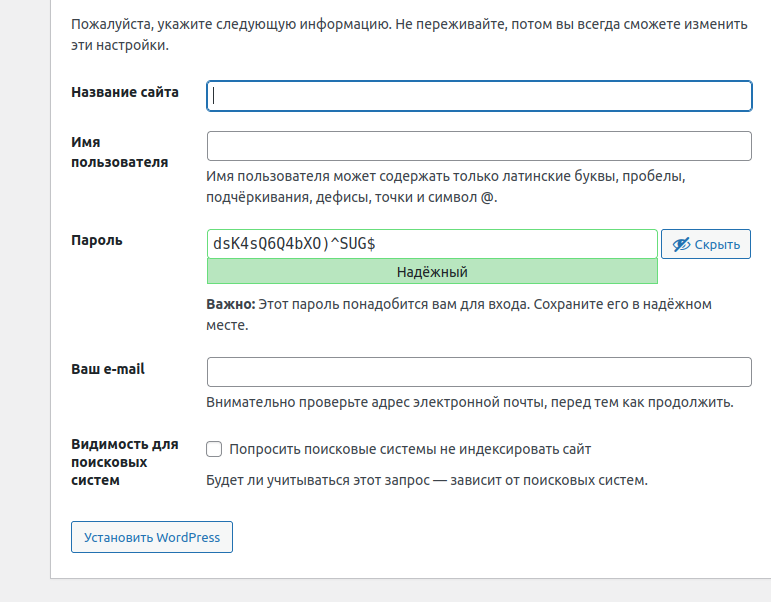
\includegraphics[width=0.7\linewidth]{lab8_1.png}
    \caption{Главная страница WordPress после установки}
    \label{fig:1}
\end{figure}

\subsection{Установка PrivateBin}
Была создана ВМ privatebin с IP-адресом 192.168.20.7. Установлен Apache, PHP, SSL, настроен виртуальный хост.

\begin{figure}[H]
    \centering
    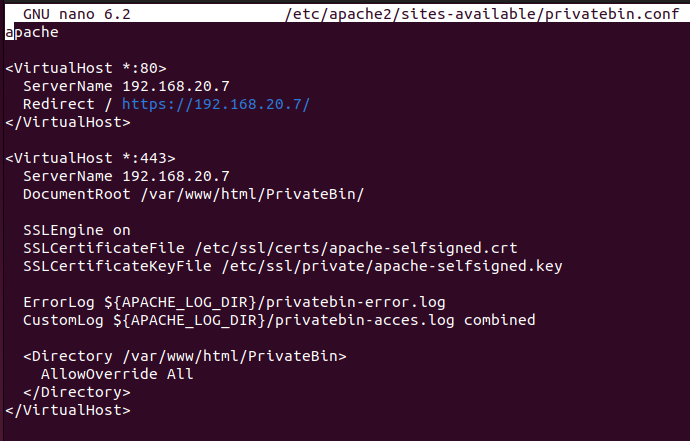
\includegraphics[width=0.7\linewidth]{lab8_2.png}
    \caption{Конфигурационный файл виртуального хоста Apache для PrivateBin}
    \label{fig:2}
\end{figure}

\subsection{Интеграция с почтовым сервером}
С помощью PrivateBin создана ссылка для безопасной передачи пароля. Ссылка отправлена по электронной почте между пользователями через почтовый сервер из лабораторной работы №7.

\section{Заключение}
В ходе работы были развернуты WordPress и PrivateBin, выполнена интеграция с почтовым сервером. Задачи выполнены в полном объеме.

\end{document}